\documentclass[a4paper,10pt]{report}
\usepackage{graphicx}
\usepackage[procnames]{listings}
\usepackage{amsmath}
\usepackage[utf8]{inputenc}

\renewcommand{\baselinestretch}{1.55}
% Title Page
\title{Learn By Doing - Fireblocks}
\author{Chinmay Lad ladchinmay@gmail.com 9757409723\\Suraj Mishra surajmishra150893@gmail.com 8976330107\\\\ \textbf{Project Mentors:}\\Deepa Avudiappan\\Rutja\\Amiraj Dhawan}


\begin{document}
\maketitle
\tableofcontents

\chapter{Abstract}
In this report, a web application based Visual Programming Language is proposed for developing a language for easier
comprehension of Firebird V code. This project aims at making expirience of children new to embedded system programming,
to grasp the concept of the Alogrithm involved rather than remebering the port configurations. 


\chapter{Objective of the Work}
The aim of this project is to develop a web application using Laravel Framework and design a Visual Programming Language for Firebird V. 
Blockly library is used for generating the blocks and parsing them to corresponding C code on the front-end.On the sever side PHP is used for parsing the XML to C code.
The final goal of this project is to deliver a web application that contains predefined blocks for writing the code for Firebird V. \\\\
\begin{tabular}{ | c | c | c |}
	\hline\hline
	\bf Sr.No & \bf Tasks & \bf Deadline \\ 
	\hline
	1.) & Install Composer, Laravel, Blockly, PHP5 & 5 days \\
	\hline
	2.) & Define blocks same as one defined in Visual & 9 days \\
	& Programming Language &\\
	\hline
	3.) & Write Code for parsing the XML file  & 8 days \\
	& to C code on server side &\\
	\hline	
	4.) & Make Execute, Save and Open Button for both & 5 days \\
	& XML and C code &\\
	\hline
	5.) & Make compiler to convert C file to hex & 6 days\\
	& and provide it for download  &\\
	\hline
	6.) & Testing/Documentation (Usage Manual, Documented Code) & 8 days
	\\ \hline

\end{tabular}

\chapter{Completion}
All the tasks have been completed. The code written using the predefined blocks correctly forms the C syntax and the hex file is also 
made and can be downloaded on the user local machine.
\section{Task-1 Install Composer, Laravel, Blockly, Xampp}
  \begin{itemize}
      \item \textbf{Composer}\\
      Run this in your terminal to get the latest Composer version:\\
	\texttt{curl -sS https://getcomposer.org/installer | php}\\
      Or if you don't have curl:\\
	 \texttt{php -r "readfile('https://getcomposer.org/installer');" | php}\\
      This installer script will simply check some php.ini settings, warn you if they are set incorrectly,\\
      and then download the latest composer.phar in the current directory.\\      
      After downloading the composer, Windows Users must set the environment path of the composer.
      For Ubuntu executed \texttt{php composer.phar install} command to install.
      \newpage
      \item \textbf{Xampp}\\
      \begin{itemize}
      \item 
      For installing the xampp application in Windows OS it is first needed to download the executable file.
      To download the installer file, got to \texttt{https://www.apachefriends.org/download.html}
      and download the appropriate file based on the operating system running. 
      \item
      The Xampp application is a Apache, MySql and PHP server used for running webapplications or webpages on the 
      localhost. The Xampp application provides with many other features like executing the applications that are already
      installed on the machine. 
      \item
      For launching any webapplication or wedpage on the server it is first required to copy the folder containing the Webpages
      to the Xampp/htdocs folder. Then go to Xampp Control Panel and start the Apache and MySQL services. Now go to webbrowser
      and type\\\texttt{localhost/Folder/index.html} or for Laravel Framework type\\ \texttt{localhost/folder/public/}\\
      \end{itemize}
      \newpage
      \item \textbf{Laravel}
      \begin{itemize}
	\item
	Laravel Framework is a PHP5 Framework used for website designs which give a structured directory arrangement. 
	Laravel attempts to take the pain out of development by easing common tasks used in the majority of web projects,
	such as authentication, routing, sessions, queueing, and caching.
	\item 
	Installing Laravel requires composer which is previously installed. Just go to terminal and type the folllowing command,\\
	\texttt{composer global require "laravel/installer=~1.1}\\
	This command installs the Laravel on the machine.
	\item
	If the framework is to be included in a project the type the command,\\
	\texttt{composer create-project laravel/laravel --prefer-dist}\\ wherein the framework is directly installed while creating a project.
	\item 
	After Installing Laravel there may be permission issues for accessing the files. Inorder to solve these problem, change the file permissions for
	storage directory by typing \texttt{chmod -R 777 /storage} by going in project directory.\\
      \end{itemize}
      \newpage
      \item \textbf{Blockly}
      \begin{itemize}
	\item
	Blockly is a library for using Visual Programming Language editors. Blockly is javascript library, using which one can
	create and define various block for a Visual Programming Language.
	\item
	To download Blockly goto,\\ \texttt{https://developers.google.com/blockly/installation/overview}
	and download from one of the three options.
	\item 
	Blockly provides generation of syntax for Javascript, Python and Dart. However any language code can be generated by 
	modifying the generators file appropriately.
	\item 
	The Library is used for mostly frontend parsing of the blocks to required code. These blocks make up a programming language that was designed around a set of principles to engage novice programmers.\\
      \end{itemize}
  \end{itemize}
  \newpage
\section{Task-2 Defining Blocks same as in Visual Programming Language}
  \begin{itemize}
   \item \textbf{Creating Blocks}\\
    \begin{itemize}
      \item 
      To generate the blocks, google-blockly provides a block-factory site where, one can easily create the blocks with desired input and names and view them.
      \item
      The block-factory provides the developer with a javascript code for the block created. This code can then added to the blocks folder in a file.
      \item
      The Visual Programming Language consisted of the custom blocks for Firebird V like forward, buzzer, left\_degrees etc. All these 
      blocks were generated and add to the blockly library using the factory.
      \item 
      Once the blocks are created they need to be stored in blocks folder. To view a block on the index page, the block tag
      is to be added to index.html file with tag type as block name.
    \end{itemize}
    
    \begin{center}
      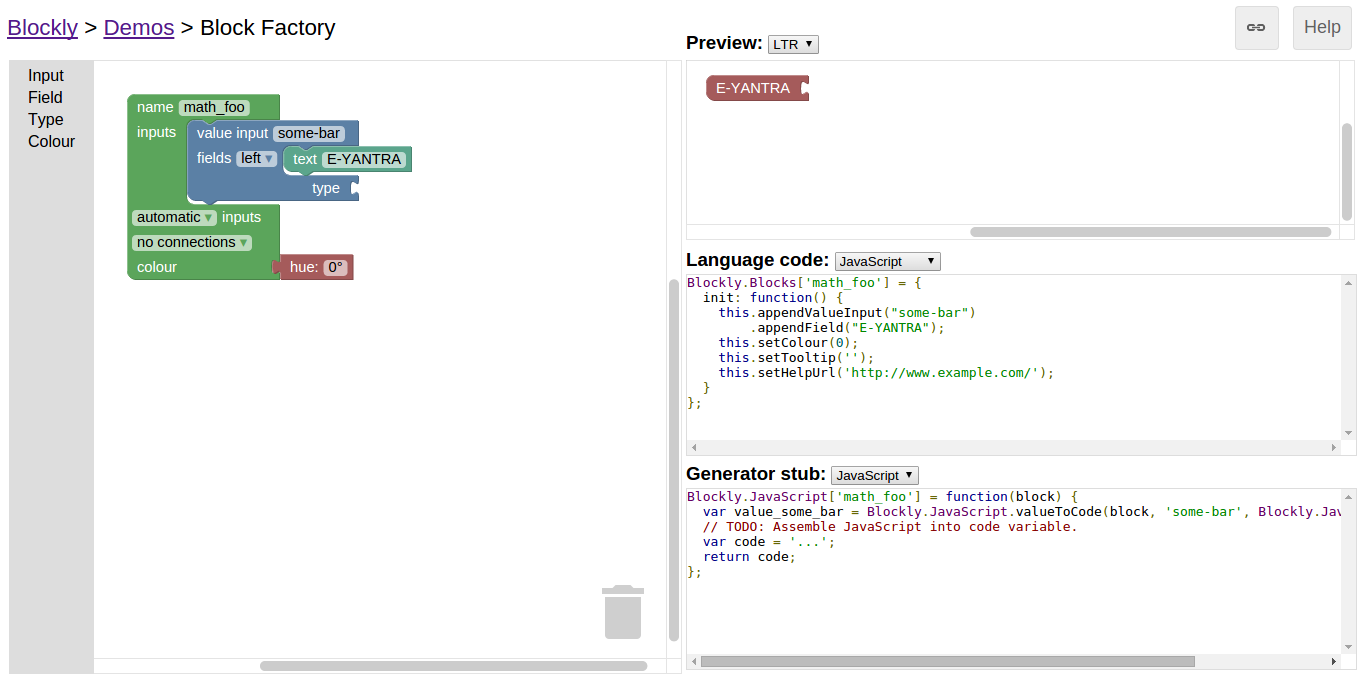
\includegraphics[scale = 0.25]{images/factory.png}\\
      \textbf{3.1 Block Factory}
    \end{center}
    \newpage
   \item \textbf{Creating Generators}\\
    \begin{itemize}
      \item
      As Blockly provides Javascript code for wach block, in the same it also provides Javascript code for parsing these blocks to requires language.
      \item
      However the Javascript genrator files provided by blockly are only for Javascript, Python and Dart.
      \item
      To make the generator files, it is necessery to know the functions related to each in the block.
      Blockly defines three such function for taking the values from the Inputs.
	\begin{itemize}
	 \item {getFieldValue(var name)}..
	 \item {valueToCode(var block, var name, var precedence)}..
	 \item {statementToCode(var block, var name)}..
	\end{itemize}
      \item
      Using these functions, values of other blocks attached to the current block can be obtained.\\
    \end{itemize}
  \end{itemize}
  \newpage
\section{Task-3 XML Parsing to C Code}
  \begin{itemize}
	\item
	For creating XML to C syntax on the server side a PHP controller is defined in which all the functions are written.
	After adding new blocks, corresponding C syntax for block on the server side is written in ParseController.php. 
	\item
	Each block contains a xml script and connecting blocks creates the corresponding script. This Xml script is used for parsing to C code on the server side.
	\item
	For XML to C parsing there are some functions similar to that in Javascript used for getting the values from connected blocks.
	 \begin{itemize}
	   \item\textbf{function xmlToCode(\$xmlDoc){...}}\\
	   Above function basically finds the childs of node and according to the no of child node, for each child node it calls the blockToCode() function,which finds the type of block (whether it is control\_if block or if\_else block etc) and calls the functions finds the type of input that it takes (like whether it takes getFieldInput() where user give the input or statementToCode() where user gives the proper statement as a input or valueToCode() where user connect some another block to given block as input) , according to that it return the equivalent parsed c code to parse function for the further process.\\
	   \item\textbf{function getFieldValue(\$block,\$name){...}}\\
	   Above function takes two input namely \$block,\$name .\$name basically gives the attribute of field node with the help of that one can find the value of input field .\\
	   \item
	   \textbf{function valueToCode(\$block,\$name){...}}\\
	   Above function takes two input namely \$block ,\$name. valueToCode() function basically takes a block as a input,so after finding the proper child of given parent node blockToCode() function called for further process.\\
	   \item\textbf{function statementToCode(\$block,\$name){...}}\\
	   Above function basically takes two arguments i.e \$block,\$input and finds the statement node and correspondingly find the value of that node.e.g control\_if blog.\\
	 \end{itemize}
  \end{itemize}
\section{Task-4 Make Execute, Save and Open \\ Button for both XML and C code}
   Whenever the user creates a project using Fireblock he/she should be able to save and restore the project. For this purpose button like
   \begin{itemize}
     \item \textbf{Save XML}\\
      This button allows the user to save the XML file to users Desktop and provide them for later use.
      The xml file is stored using a javascript code save.js
     \item \textbf{Open XML}\\
     To restore the previous project the user can upload the xml file to the server and the server then can restore the blocks that the user had been working on.
     To do so we make use of openButton javascript code which opens the dialogue for s
     \item \textbf{Save C}\\
     Once the user has finished implementing the algorithm he/she can save the C code visible in FirebirdV Tab into file on the local machine
     \item \textbf{Execute}\\
     Once the algorithm is implemented using the blocks the user can then verify and click the Execute button and then if the alogrithm is free of errors
     then a hex file will be made available for download. Clicking this button executes a parse.js function in which send the xml text to the server for parsing.
   \end{itemize}
\newpage
\section{Task-5 Make compiler to convert C file to hex and provide it for download} 
    The main task of the web application is to provide a hex file to download. To do so, after completing the impletmentation of the the algorithm,
    user clicks on the execute button; this sends the control to parse.js after compiling. 
\chapter{Results and Discussion}
    In this Project we have used Laravel Framework for efficient and elegant handling of server.
    On opening the Webpage of this site, it redirects to Fireblocks.blade.php. Using Blade Templating the header contents are defined in FireBlocks.blade.php
    and the main body is contained in blocks.blade.php. The blocks.blade.php file contains the html code for blocks that are visible.
    The blocks are divided into categories which are named according to their types. \\
    The Web application is divided into 3 phases-
    \begin{itemize}
     \item Blocks
     \item Front End C Code.
     \item Back End C Code.
    \end{itemize}
    The workflow of the application goes through all this 3 phases for final hex file generation.\\
   \section{Blocks}
    In this phase the the user designs the algorithm using the predefined blocks that are provided on the side tab.
    This blocks when draggesd onto the workspace, an xml code is generated in tandem of corresponding block which gives information regarding the same.\\
    XML provides information about each block and the structure of the XML  gives the information about the connections of the blocks.
    \begin{center}
    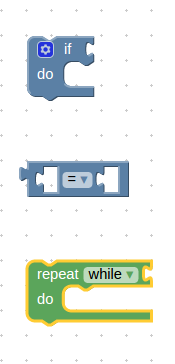
\includegraphics[scale =0.6]{images/blocks.png}\\[.3in]
    \textbf{Blocks on Workspace}\\[1.3in]
    \end{center}

    \begin{center}
    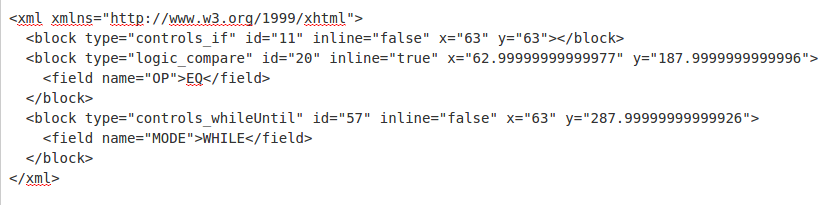
\includegraphics[scale =0.5]{images/xml.png}\\[.3in]
    \textbf{Corresponding XML Syntax}
    \end{center}
    \newpage
    \section{Front-End C Code}
    After the user has finished with the algorithms using blocks he/she can verify the code formed by the blocks.
    FirebirdV tab when clicked displays the C code genrated by the blocks. This code is structured according to the XML structure.
    Front End  C code parsing is done by using Blockly library. \\
    
    \begin{center}
    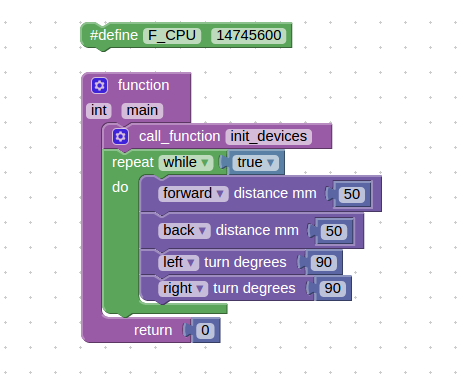
\includegraphics[scale =0.6]{images/code.png}\\[.1in]
    \textbf{Blocks on Workspace}\\[1in]
    \end{center}

    \begin{center}
    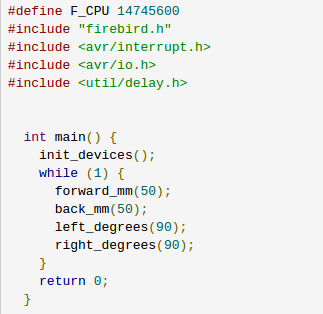
\includegraphics[scale =0.5]{images/firebirdV.png}\\[.1in]
    \textbf{Corresponding C Syntax}
    \end{center}

\chapter{Bugs}
Something
\chapter{Future Work}
  This application has a very wide scope.
  \begin{itemize}
   \item Automatic Hex Loading on the Robot from server.
   \item Addition of more abstraction for easier understanding.
   \item More usefuk functions.
  \end{itemize}

\chapter{References}
\begin{itemize}
 \item Laravel Documentation: http://laravel.com/docs/5.0
 \item Hex File Generation: http://www.engineersgarage.com/forums/avr/how-generate-hex-file-using-avr-gcc-commands
 \item For PHP parsing refer: http://php.net/manual/en/class.domdocument.php
 \item To understand tree structure of xml: (http://www.w3schools.com/xml/xml\_tree.asp
 \item To understand javascript parsing: http://www.w3schools.com/xml/xml\_parser.asp
 \item To make blocks: https://blockly-demo.appspot.com/static/demos/blockfactory/index.html
 \item Blockly: https://developers.google.com/blockly/custom-blocks/block-factory
 \item Save and upload file: https://developer.mozilla.org/en/docs/Web/API/FileReader
\end{itemize}

\end{document}          
